\documentclass[12pt]{report}

\usepackage[utf8]{inputenc}
\usepackage[T1]{fontenc}
\usepackage[magyar]{babel}

\usepackage{times}

\usepackage{amsmath}
\usepackage{amssymb}
\usepackage{amsthm}

\usepackage{fancyhdr}

\usepackage{graphicx}
\usepackage{psfrag}

\usepackage{listings}

\usepackage{url}

\usepackage{setspace}

\usepackage{enumitem}

\newtheorem{tét}{Tétel}[chapter]
\newtheorem{defi}[tét]{Definíció}
\newtheorem{lemma}[tét]{Lemma}
\newtheorem{áll}[tét]{Állítás}
\newtheorem{köv}[tét]{Következmény}

\theoremstyle{definition}
\newtheorem{megj}[tét]{Megjegyzés}
\newtheorem{pld}[tét]{Példa}

%Margók:
\hoffset -1in
\voffset -1in
\oddsidemargin 35mm
\textwidth 150mm
\topmargin 15mm
\headheight 10mm
\headsep 5mm
\textheight 237mm

\begin{document}

%A FEJEZETEK KEZDÕOLDALAINAK FEJ ES LÁBLÉCE:
%a plain oldalstílust kell átdefiniálni, hogy ott ne legyen fejléc:
\fancypagestyle{plain}{%
%ez mindent töröl:
\fancyhf{}
% a láblécbe jobboldalra kerüljön az oldalszám:
\fancyfoot[R]{\thepage}
%elválasztó vonal sem kell:
\renewcommand{\headrulewidth}{0pt}
}

%A TÖBBI OLDAL FEJ ÉS LÁBLÉCE:
\pagestyle{fancy}
\fancyhf{}
\fancyhead[L]{Videólejátszó alkalmazás idegen nyelvet tanulóknak}
\fancyfoot[R]{\thepage}


%A címoldalra se fej- se lábléc nem kell:
\thispagestyle{empty}

\begin{center}
\vspace*{1cm}
{\Large\bf Szegedi Tudományegyetem}

\vspace{0.5cm}

{\Large\bf Informatikai Intézet}

\vspace*{3.8cm}


{\LARGE\bf Videólejátszó alkalmazás idegen nyelvet tanulóknak }


\vspace*{3.6cm}

{\Large Szakdolgozat}

\vspace*{4cm}

%Értelemszerûen megváltoztatandó:
{\large
\begin{tabular}{c@{\hspace{4cm}}c}
\emph{Készítette:}     &\emph{Témavezetõ:}\\
\bf{Krucsai Attila}  &\bf{Tóth Zotán Gábor}\\
programtervező informatikus     &egyetemi tanársegéd\\
szakos hallgató&
\end{tabular}
}

\vspace*{2.3cm}

{\Large
Szeged
\\
\vspace{2mm}
2019
}
\end{center}


%A tartalomjegyzék:
\tableofcontents


\chapter*{Feladatkiírás}
%A tartalomjegyzékben mégis szerepeltetni kell, mint szakasz(section) szerepeljen:
\addcontentsline{toc}{section}{Feladatkiírás}
\spacing{1.5}


Az idegennyelv tanulás folyamán sokszor nemcsak a tankönyvekből tanulunk. Az internet, könyvek, újságok, filmek mind szerves részét képezhetik egy idegennyelv elsajátításának. A szoftver azoknak az egyéneknek nyújthat segítséget, akik rendszeresen néznek idegennyelvű filmeket, idegennyelvű felirattal. A felhasználó egy ismeretlen szó esetén megállíthatja a lejátszást, és a mondatelemre kattintva megtudhatja az anyanyelvi jelentését. Így a szótározással eltöltött idő lényegesen kevesebb, kevésbé szakad meg a film folyamatossága.
Az ismeretlen szavakat az alkalmazás egy adatbázisban tárolja, amelyből a film befejeztével egy szószedet generálódik a filmből kiragadott példamondatokkal. A létrejött fájlt el lehet menteni, így a felhasználó a későbbiekben is átnézheti a nehezebben megjegyezhető szavakat.
Egy másik lehetőség a film véget értével, hogy az alkalmazás egy feleletválasztós kvízt generál, amely a korábban ismeretlen mondatelemeket tartalmazza. A tanuló így ellenőrizheti a saját tudását, valamint azt, hogy mennyire sikerült elsajátítania az idegen szavak jelentéseit.


\chapter*{Tartalmi összefoglaló}
\addcontentsline{toc}{section}{Tartalmi összefoglaló}

A tartalmi összefoglalónak tartalmaznia kell (rövid, legfeljebb egy oldalas, összefüggõ megfogalmazásban)
a következõket: a téma megnevezése, a megadott feladat megfogalmazása - a feladatkiíráshoz viszonyítva-,
a megoldási mód, az alkalmazott eszközök, módszerek, az elért eredmények, kulcsszavak (4-6 darab).

Az összefoglaló nyelvének meg kell egyeznie a dolgozat nyelvével. Ha a dolgozat idegen nyelven készül,
magyar nyelvû tartalmi összefoglaló készítése is kötelezõ (külön lapon), melynek terjedelmét a TVSZ szabályozza.

\chapter*{Bevezetés}
\addcontentsline{toc}{section}{Bevezetés}
\spacing{1.5}
Szakdolgozatom célja, egy a nyelvtanulást elősegítő videolejátszó alkalmazás fejlesztése, melynek segítségével a felhasználók a szórakozást tanulással köthetik össze. Ennek eredményeképp úgy tudnak elsősorban idegennyelvű szavakat elsajátítani, hogy mellőzik a tanulással járó feszültséget, illetve kötöttséget. Tehát a nyelvek szókincsének elsajátítása, elmélyítése, tudatosítása, lehető legbiztonságosabb használata ezáltal könnyedebbé, szórakoztatóbbá és gördülékenyebbé válhat, mely egy hatékonyabb tanulási folyamatot tesz lehetővé. Mivel az általam elkészített alkalmazás elsősorban filmek lejátszására ajánlott, így a felhasználok egy sokkal inkább a hétköznapi kommunikációhoz alkalmazható szókincsre tehetnek szert. Ezen szoftver segítségével az idegennyelv-tanulástól ódzkodó személyek érdeklődése nagymértékben felkelthető, mivel a tanulás nem direkt módon, hanem filmnézés, szórakozás közben történik, a szavak az idegennyelven hallott és látott szövegben, kontextusban rögzülnek. 

Napjainkban egyre inkább felmerül a kérdés, hogy a nyelvtanulást milyen módszerekkel lehet hatékonyabbá, illetve játékosabbá tenni. Kétségtelen azonban, hogy egy idegen nyelv magabiztos szintű elsajátításához a megfelelő méretű szókincs birtoklása elengedhetetlen. A szavak memorizálása sokszor monoton folyamat, valamint rengeteg ráfordított időt igényel. Ennek kapcsán saját tapasztalatból is biztonsággal állíthatom, hogy az idegen nyelvű szavak elsajátítása megítélésem szerint a jelenleg használatos oktatási módszerekkel igen monoton, mely a diákok motiválatlanságát, elidegenülését eredményezheti. Mivel a motiváció hiánya gyakran tanulási nehézségeket eredményez, a nagy erőfeszítések árán megtanult szavak nem rögzülnek megfelelően, ha igen, akkor sokszor hibásan, így gyorsan el is felejtődnek. A jelenlegi, fejlett informatikai világban a fiatal generáció mindennapi életében természetes és elengedhetetlen az informatikai eszközök használata, ami lehetővé teszi az idegennyelv tanulás elősegítését is. Az informatikai eszközök sokoldalúsága, hordozhatósága, a nap minden órájában lehetővé teszi a használatot, amely a filmnézéssel és szórakozással egybekötött nyelvtanulást is elősegíti, így a fiatal generáció életvitelébe teljes mértékben beilleszthető.
 Egy alternatívaként merülhet fel a tanulásra az a videolejátszó alkalmazás, amelyet szakdolgozatom keretein belül készítettem el, azt a célt kitűzve magam elé, hogy közelebb hozzam egymáshoz a tanulást és a szórakozást. 

Egy idegennyelv elsajátítása során sokszor nemcsak tankönyveket használunk. Az internet, könyvek, újságok, filmek mind szerves részét képezhetik a tanulásnak. A szoftver azoknak az egyéneknek nyújthat nagymértékben segítséget, akik rendszeresen néznek idegennyelvű filmeket, idegennyelvű felirattal. A felhasználó egy a számára ismeretlen szó esetén a film megállítása nélkül a mondatelemre kattintva megtudhatja az anyanyelvi jelentését. Így a szótározással eltöltött idő megszűnhet, mely eredményeképp a megtekintett film folyamatossága biztosított. Azon szavakat, melyek anyanyelvi megfelelőjét a felhasználó filmezés közben megtekinti, az alkalmazás egy adatbázisban tárolja, amelyből a film befejeztével egy szószedet generálódik. Az így összeállt lista különlegessége, hogy nem csak az egyes szavak idegen- illetve anyanyelvű alakjait tartalmazza, hanem ezeket a filmből kiragadott példamondatokkal, abban a kontextusban szemlélteti, amelyben az adott szó korábban előfordult. A létrejött fájl automatikusan mentésre kerül a felhasználó eszközére, így a későbbiekben is megtekinthetővé válik a lista. Egy további opcióként kínálkozik az a lehetőség, hogy a film végeztével az alkalmazás egy feleletválasztós kvízt generál azokból a mondatelemekből, melyeket a felhasználó korábban ismeretlenként jelölt meg. Ezáltal lehetősége nyílik a megszerzett tudás ellenőrzésére is.

Alkalmazásom célja tehát egy olyan alternatív lehetőség felkínálása az idegennyelvet tanulók részére, amellyel az ismeretlen szavak memorizálása szórakozással köthető össze, amely által az idegennyelv elsajátításával járó stressz csökkenthető, esetlegesen elkerülhetővé válik, így nagy eséllyel sikerélmény keletkezik, ezáltal tanulás hatékonysága is nő.

\chapter{Háttér}
\addcontentsline{toc}{section}{Háttér}
\spacing{1.5}
Az alkalmazás elkészítése előtt kutatást végeztem a témában lehetséges alternatívaként felmerülő szoftverekről. Ezen kutató, illetve háttérmunkát rendkívül fontosnak tartom, hiszen ezáltal betekintést nyerhetünk a piaci igényekbe, következtetéseket vonhatunk le a már elérhető programok palettájából. A kutatás során elsődleges forrásként az internetet használtam, tehát a jelen dolgozatban bemutatott opciók nagy részben weboldalakról származnak. Itt rengeteg hasonló célokat szolgáló szoftver, honlap található, azonban ezek funkcionalitása eltér az általam fejleszteni kívánt alkalmazástól. Továbbá fontosnak tartom megemlíteni azt a tényt is, hogy az előzőekben említett, általam elkészítendő alkalmazás ingyenesen elérhető lesz, szemben a világhálón található hasonló alkalmazásokkal.

Kutatásom első részében olyan programokat kínáló megoldásokat kerestem, melyek képesek a feliratfájlok szövegét felismerni, valamint lefordítani. Erre számtalan online alkalmazás, illetve felület képes. Ezek a megoldások többnyire ingyenesek, mivel a weblapok rendszerint nagyméretű reklámfelületeket tartalmaznak. A működésük egyszerű: a felhasználó vagy drag\&drop módszerrel, vagy tallózással kiválasztja az általa lefordítani kívánt megfelelő kiterjesztésű fájlt, amelyet feltölt a weboldalra. Ezután a képernyőn pillanatok alatt megjelenik az eredeti, valamint a lefordított szöveg. A felhasználó itt kiválaszthatja, módosíthatja a fordítás nyelvét, mind a fordítandó, mind pedig a fordított nyelvet. Legtöbbször nyelvfelismerő szolgáltatás is működik, amely nagy biztonsággal képes meghatározni a forrásfájl nyelvét, ezzel is gyorsítva a fordítás folyamatát. Ha a felismerő hibázna lehetőség van manuálisan is megadni a nyelvet. Ezen megoldások nagy előnye, hogy gyorsak, könnyedén elérhetőek, illetve nem szükséges semmiféle külön alkalmazás telepítése a számítógépre. Működésükhöz csupán egy böngésző, valamint internetkapcsolat szükségeltetik, így ezek akár mobileszközökön is használhatók. E megoldás nagy hátránya a pontatlanság, mivel a szöveget online fordítók segítségével alakítja át az alkalmazás. Az így keletkezett mondatok legtöbbször helytelenek, sok bennük a nyelvtani hiba, legtöbbször értelmetlenek. További hátrányuk, hogy működésükhöz elengedhetetlen az internetkapcsolat. Mivel fordításhoz feliratfájl feltöltése szükséges, így ebből adódóan gyenge internetelérés esetén a sebességük drasztikusan lecsökkenhet.

Egy másik opcióként kínálkoznak a fentebb említett megoldáshoz nagyon hasonló szoftverek. Működésük majdnem analóg az online szövegfordítókkal, azonban lényeges különbség, hogy a fordítást videolejátszás közben is képes végrehajtani. Online ingyenesen elérhetőek, telepítést követően teljes értékű videolejátszó alkalmazásként képesek funkcionálni. Megfelelő médiafájl kiválasztása után lehetőség van feliratok fájlból történő megjelenítésére is. Az alkalmazás online fordítók segítségével alakítja át az eredeti szöveget a célnyelvre. Működésük gyors, hatékony, azonban felhasználói felületük sokszor hiányos, nem felel meg a mai kor elvárásainak. Továbbá, mivel a felirat sorait egyben kezelik, így a fordítások legtöbbször pontatlanok, hiányosak, valamint nyelvtanilag helytelenek. Fő előnyük tehát, hogy filmnézés közben is képes lefordított feliratokat megjeleníteni úgy, hogy nem szükséges a feliratokat előzőlegesen lefordítani. Egyes fajták arra is lehetőséget biztosítanak a felhasználónak, hogy a filmhez saját fordításokat készítsen. Mivel a használatukhoz az alkalmazást kötelező telepíteni a számítógépre, így működéséhez csak akkor szükséges internetkapcsolat, amikor a fordítás történik. Ekkor kevesebb az adatforgalom, mint az előzőleg említett megoldásnál, mivel nem szükséges fájlok feltöltése egy külső szerverre. Hátrányként megemlíthető az a tény, hogy a szoftverek a feliratokat csak egészben, legfeljebb soronként tudják lefordítani, így a keletkező szöveg rendkívül pontatlan.

\section{Architekturális áttekintés}

Kutatás után az alkalmazás megvalósításához szükséges technológiákat gyűjtöttem össze. Mivel ezt egy asztali, telepíthető szoftvernek szántam, így a \textit{Java} nyelv, azon belül is a \textit{Java 8} mellett döntöttem. A választás azért előnyös, mivel a nyelv platformfüggetlen, így különböző operációs rendszerekre is telepíthető lesz az alkalmazás, valamint nagy mennyiségű API-k állnak rendelkezésre. A projekt, illetve a függőségek kezelésére \textit{maven 3.6.0}-as verzióját használtam. A külső könyvtárak kezelése ezzel  gyorsabbá, egyszerűbbé válik. A szoftver videolejátszó funkcióit a \textit{vlcj} keretrendszer segítségével valósítottam meg, amely a népszerű \textit{VLC} videolejátszó alkalmazáshoz egy natív hívásokkal operáló \textit{API}, amely segítségével lehetőség nyílik a \textit{VLC} funkcionalitásait \textit{Java} nyelven használni. A program grafikai felülete \textit{Java Swing} segítségével íródott, s mivel a \textit{vlcj} is támogatja az ebbe történő beágyazást, így egyszerű volt azt kiegészíteni, továbbfejleszteni. Az adatok tárolására szükségem volt egy adatbázis kezelő rendszerre. Mivel a a szükséges adatbázis struktúra egyszerű, illetve az elvégzendő műveletek tárháza csekély, ezért végül a \textit{H2} adatbázist választottam. Ennek nagy előnye, hogy képes \textit{in-memory} adatbázis kezelésére, valamint a használatához nem szükséges további csomagok feltelepítése a számítógépre, egyszerűen a megfelelő \textit{.jar} fájl importálásával elérhetővé válik az adatbázis. A program egyik legfontosabb funkciója, a szavak, mondatelemek fordítása a \textit{Microsoft Translate API} beiktatásával valósult meg. Az API képes több, mint 60 nyelvfelismerésére, illetve fordítására. Használata egyszerű, működése gyors, pontos, illetve ami még fontos volt a projekt szempontjából, hogy képes egynél több találat megjelenítésére is.

A fejlesztés \textit{Windows 10} operációs rendszer alatt történt. A programozáshoz, futtatáshoz, teszteléshez \textit{IntelliJ IDEA} integrált fejlesztői környezetet használtam. A szoftver verziókövetése, illetve a fájlok tárolása \textit{GitHub} repository-n keresztül valósult meg.
\chapter{Az alkalmazás funkcionalitásai}

\section{Videólejátszó alapfunkciók}
A alábbi fejezetben az elkészült alkalmazás főbb funkcióit mutatom be, fejtem ki részletesen, külön kitérve a fontosabb, érdekesebb részekre.

A szoftver alapját, magját adó komponens a \textit{VLC} java-n alapuló keretrendszer segítségével valósult meg. Első lépésként a \textit{VLC} videólejátszó megfelelő operációs rendszerre való feltelepítése szükséges. Windows esetén lehet 32 illetve 64 bites verzió. E lépést kötelező megtenni, mivel az fejlesztett alkalmazás a \textit{VLC} lejátszó funkcióit veszi igénybe, nélküle a szoftver nem működik. Ezután a vlcj nevű open source projektet vettem igénybe. Ez Java könyvtárakat ad a \textit{VLC} média lejátszóhoz, így annak majdnem az összes natív funkciója elérhetővé válik a \textit{LibVLC}-n keresztül. Ezen kívül egy keretrendszer használatát is elérhetővé teszi, amely egy egyszerű, magas szintű programozási modellt biztosít, ami magába foglalja a natív könyvtárakhoz való hozzáférést. E keretrendszer amennyire csak lehetséges megvédi a felhasználóját az eredeti könyvár helytelen használatától, ami akár a fejlesztett alkalmazás összeomlását is okozhatja. Segítségével a fejlesztés magas szinten történhetett. Az alkalmazás elindítása után egy egyszerű videó lejátszó kezelőfelülete tárul elénk, amely a \ref{fig:main_screen} ábrán látható.
  
\begin{figure}
\centering
  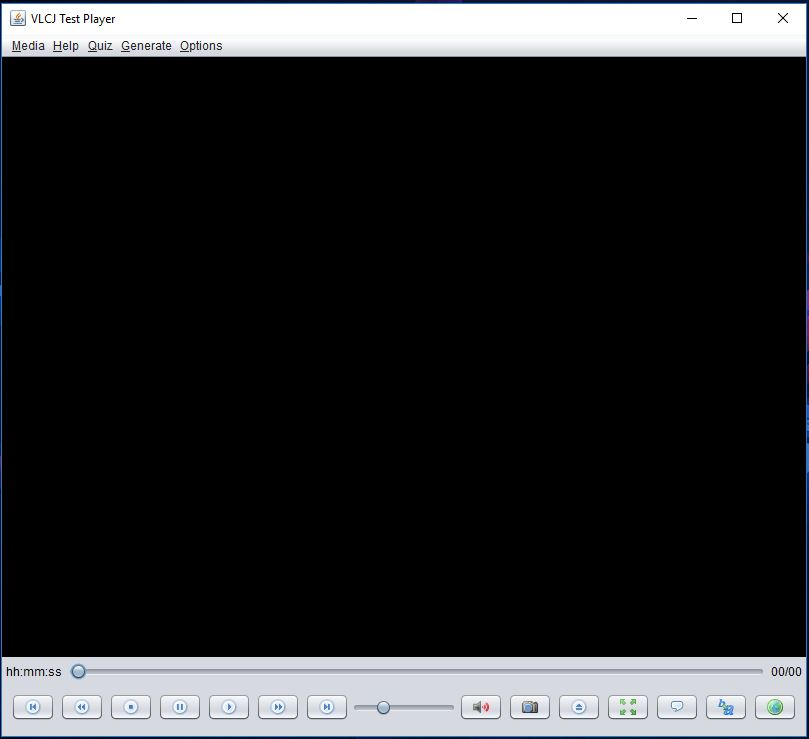
\includegraphics[width=.8\linewidth]{images/main_screen.jpg}
  \caption{Az alkalmazás kezelőfelülete}
  \label{fig:main_screen}
\end{figure}

A képernyő bal alsó sarkában találhatóak meg a videó lejátszását szabályozó gombok. Ezek rendre az előző fejezet, visszatekerés, megállítás, pillanatmegállítás, indítás, előre tekerés, valamint következő fejezet. Középen egy csúszka kapott helyet, amely a hangerőszabályzást teszi lehetővé. Ettől jobbra találhatóak a némító, képernyőfelvétel, médiaválasztó, teljes képernyő, felirat választó, fordítás nyelve, illetve az online feliratok gombok. Ezek működéséről későbbi fejezetekben írok részletesen. Feljebb helyezkedik el a keresősáv, és egy számláló balra, valamint egy jobbra. A bal számláló a lejátszott videó aktuális időpillanatát jelzi, másodperces pontossággal. A csúszka segítségével egyszerűen, intuitívan tekerhetünk a videóban. A jobboldali számláló az aktuális fejezetet mutatja. Az alkalmazás felső részén a menüsáv található, rajta öt különböző menüponttal. Az első segítségével médiafájlokat tallózhatunk, illetve kiléphetünk a szoftverből. A második lehetőség egy segítség opció, a harmadik az ellenőrző kvíz kitöltését teszi lehetővé. A \textit{generate} menüt kibontva PDF fájlt generálhatunk az általunk ismeretlennek vélt szavakból. Felül az utolsó lehetőség a beállítások menüpont, ahol a felirat méretét, illetve késleltetését állíthatjuk be milliszekundumos pontossággal. Ezek áttekintése után már tudunk média fájlokat hozzáadni a szoftverhez. Ehhez kattintsunk az \textit{Eject} gombra az alsó panelről, vagy válasszuk a \textit{Media}, \textit{Play File…} menüpontot. Ekkor megnyílik a felhasználó előtt egy tallózó ablak, ahol böngészhetünk a saját fájlrendszerünkben. Alap beállítás szerint csak a média fájlok jelennek meg az ablakban, azonban ez bármikor felülírható. Itt lehetőség van keresésre, részletes, vagy listás megjelenítésre, feljebb navigálásra, főoldalra való visszatérésre A szoftver képes rengeteg különböző kódolású videó-, és hangfájl lejátszására. Kilépésre a \textit{Cancel} gomb megnyomásával van lehetőség. Ha megtaláltuk a nekünk megfelelő fájlt, a \textit{Play} gombra való kattintással kezdhetjük el a lejátszást. Az ablakot bármikor átméretezhetjük, amivel a benne lejátszott tartalom is méretet vált, fekete sávokkal kitöltve a képaránynak nem megfelelő részeket. Lehetőségünk van a lejátszó némítására, a \textit{Toggle Mute} gombra való kattintással. Ezzel egy időben a gomb ikonja is a megfelelő állapotba vált, jelezve ezzel, hogy a lejátszás le van-e némítva, vagy sem. Az ezt megvalósító kódrészlet \ref{lst:mute}.
\begin{lstlisting}[caption=Némítást implementáló kódrészlet, language=java, label={lst:mute}]
toggleMuteButton.addActionListener(new ActionListener() {
    @Override
    public void actionPerformed(ActionEvent e) {
        mediaPlayer.mute();
        if(mediaPlayer.isMute()){
            toggleMuteButton.setIcon(new ImageIcon(getClass()
            .getClassLoader()
            .getResource("icons/sound.png")));
        } else {
            toggleMuteButton.setIcon(new ImageIcon(getClass()
            .getClassLoader()
            .getResource("icons/sound_mute.png")));
        }
    }
});
\end{lstlisting}


\section{Teljes képernyős mód}

Az eddig elkészült alkalmazás már képes videofájlok lejátszására, illetve alapvető vezérlési funkciókat is ismer, azonban a szoftver egy fontos része hiányos, tekintve, hogy elsősorban film lejátszására ajánlott. Ez pedig a teljes képernyős mód. Az alkalmazás, amint a felhasználó megnyomja a teljes képernyős mód gombot, kitölti a képernyőfelület egészét, eltüntetve ezzel a menüsávot és a kezelőpanelt.

Az új funkció alkalmazása azonban egy új problémát vetett fel: ha a képernyő egésze foglalt, és nem jelenik meg a kezelősáv, akkor a felhasználó nem tudja a teljes képernyős módot bezárni. Ennek megoldására egy általánosan használt módszert alkalmaztam. Ha a felhasználó a kurzort a képernyő alsó felére húzza, a vezérlőpanel megjelenik, és megjelenítve is marad mindaddig, amíg a felhasználó el nem távolítja az alsó területről a kurzort. Itt egyszerűen a teljes képernyős mód gombjára kattintva kiléphetünk abból. Ennek a megvalósításáért, illetve a panel megjelenítésének kezeléséért egy \textit{MouseListener} felel. Amennyiben az alkalmazás teljes képernyős módban van, a figyelő ellenőrzi a kurzor aktuális Y koordináta szerinti pozícióját, és ha ez egy bizonyos szám alatti, vagy feletti, akkor a szerint jeleníti meg, valamint rejti el a vezérlőpanelt, illetve ennek megfelelően igazítja a vásznat és a feliratokat (\ref{lst:mouselistener}).

\begin{lstlisting}[caption=A \textit{MouseListener} megvalósítása, label={lst:mouselistener}, language=java]
@Override
public void mouseMoved(MouseEvent e) {
   if(mediaPlayer.isFullScreen()) {
        if (e.getYOnScreen() < Toolkit
            .getDefaultToolkit()
            .getScreenSize().height-5
        && controlsPanel.isVisible()) {
            controlsPanel.setVisible(false);
            ((SubtitleOverlay)(mediaPlayer.getOverlay()))
            .decreaseYOffset(controlsPanel.getHeight());
        } else if (e.getYOnScreen() >= Toolkit
            .getDefaultToolkit()
            .getScreenSize().height-5
        && !controlsPanel.isVisible()) {
            controlsPanel.setVisible(true);
            ((SubtitleOverlay(mediaPlayer.getOverlay()))
            .increaseYOffset(controlsPanel.getHeight());
        }
    }
}
\end{lstlisting}

Ezen felül további kényelmi funkciókat is implementáltam a hatékonyabb teljes képernyős mód kezeléséért. A mód aktiválható a vászonra történő dupla kattintással, és meg is szüntethető ugyanezzel a módszerrel. Ehhez szintén egy \textit{MouseListener}-t hívtam segítségül, amely figyeli az egymás utáni kattintások számát, és ha ez az érték kettővel egyenlő, be- valamint kilép a teljes képernyős módból. Egy másik megvalósított segédfunkció az \textit{Esc} gombbal történő vezérlés. Amennyiben az alkalmazás teljes képernyőn fut, a mód megszakítható az \textit{Esc} gomb egyszeri megnyomásával. Mindkét lehetőség kényelmesebb, gyorsabb használatot tesz lehetővé, ezzel is növelve a felhasználói komfortérzetet.


\section{Média- és feliratfájlok választása}

\begin{figure}
  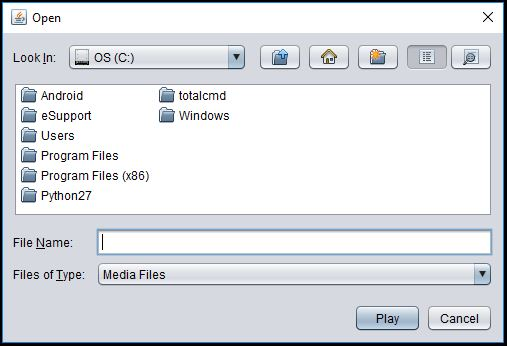
\includegraphics[width=\linewidth]{images/chooser_screen.jpg}
  \caption{Médiafájl választó}
  \label{fig:chooser_screen}
\end{figure}

A médiafájlok lejátszása a videólejátszó alkalmazás elengedhetetlen részét képezik, hiszen enélkül a felhasználó képtelen lenne, vagy csak komplikált módszerek igénybevételével tudná megtekinteni videó fájljait. A feliratok megjelenítése a szoftver egy másik sarkallatos pontja. E funkció teszi lehetővé a felhasználó számára, hogy filmjeit idegennyelven feliratozva tekinthesse meg. Mindkettő megvalósítása egy tallózó segítségével történik, amely a megszokott módon, gyorsan, kényelmesen enged utat a fájlválasztásnak. Alapesetben a választó a felhasználó \textit{home} könyvtárában nyílik, onnan navigálva kereshetők a tartalmak. A fájlok kiválasztása után azok azonnal megjelennek a képernyőn, valamint videó fájlok esetén el is indulnak. A tallózók megvalósítása \textit{Java Swing} komponensek, azon belül \textit{JButton}, \textit{JFileChooser} segítségével történtek. A médiafájl választás folyamata a \textit{Load/Eject media} gomb megnyomásával indítható el, amely a vezérlőpanel jobb alsó részén elérhető. A gombhoz használt ikont a \textit{resources/icons} könyvtárból importáltam. A fájlválasztáshoz a könnyebb használat érdekében szűrőket definiáltam, amelyek a fájlok kiterjesztése alapján szűrik meg az éppen aktuális könyvtár tartalmát, és jelenítik meg csak azokat az elemeket, amelyek a feltételnek megfelelnek. Ezek külön-külön a videó, audió, lejátszási lista, illetve a médiafájlokra való szűrést teszik lehetővé. Ezeken felül elérhető egy \textit{All files} opció is, amely filterezés nélkül az összes elérhető fájlt kilistázza a felhasználó számára. Ezen szűrőket a fájlválasztó \textit{Files of Type} címke mellett található legördülő listából választhatjuk ki. Amennyiben ennél specifikusabb módon szeretnénk keresni, lehetőségünk van a keresőmező használatára. Ezt a \textit{File Name} felirat mellett található mezőbe írt kulcsszavak segítségével tehetjük meg. Ha gyorsabba szeretnénk navigálni a könyvtárak között, ezt megtehetjük a választó felső részén fellelhető legördülő listából kiválasztható elemekkel. Itt megtalálhatók a számítógépen elérhető fő könyvtárak, mint például a különböző meghajtók, asztal és egyéb nagyobb méretű mappák. A lista helyzetétől jobbra felfedezhető néhány további gomb. Ezek rendre: egy szinttel feljebb lépés a könyvtárhierarchiában, vissza a \textit{home} könyvtárba, új mappa létrehozása, lista- illetve részletes nézet közötti váltás. Ha megtaláltuk az általunk lejátszani kívánt fájlt, kijelölés után a \textit{Play} gomb megnyomásával, illetve a fájlon történő dupla kattintással indíthatjuk el azt. Ugyanezen komponens használatával valósítottam meg a feliratfájlok kiválasztásának kezelését is. Az ablakot a kezelőpanelen fellelhető \textit{Select subtitle} gombra történő kattintással jeleníthetjük meg. A különbség csupán annyi a két ablak között, hogy a feliratfájl-választó ablakban más szűrők definiáltak. Ez értelemszerűen a feliratfájlok kizárólagos megjelenítésére ad lehetőséget. Mindkét ablak esetében kényelmi funkcióként implementálásra került az elérési útvonal megjegyzése. Amikor a felhasználó fájlt választ, legyen a média, vagy felirat, az alkalmazás elmenti a fájl elérési útvonalát, és ez alapján állítja a tallózó az aktuális kiinduló könyvtárát (\ref{lst:aktualis_konyvtar}).

\begin{lstlisting}[caption=Aktuális könyvtár beállítása, label={lst:aktualis_konyvtar}, language=java]
	if(actualFile != null)
	    {fileChooser.setCurrentDirectory(actualFile);
	}
\end{lstlisting}
        
Ebben a néhány kódsorban mindösszesen annyi történik, hogy amennyiben az aktuális fájl, azaz az utolsóként kiválasztott fájl nem üres, akkor a tallózó aktuális könyvtára a fájlt tartalmazó mappa lesz. Ugyanez a kódrészlet megtalálható a feliratfájl választó kódjában is. Mindezeken felül a fájlválasztó másik módon is megjeleníthető. A felső menüsávban a \textit{Media} menüpont alatt található \textit{Play Media…} menü kiválasztásával a tallózó megjelenik a képernyőn. Itt akár gyorsbillentyűvel, úgynevezett mnemonikkal is hatékonyabbá tehetjük a fájlválasztást elindítását. A menüsávban található \textit{Media} az \textit{"m"}, a \textit{Play File…} menü pedig az \textit{"f"} billentyűk lenyomásával hívható elő.
 Az implementált két tallózó a fent említett részletek alapján alkalmas fájlok gyors és hatékony szelekciójára, olyan módon, hogy azt egy átlagfelhasználó is könnyedén, kevés kutatással megteheti.

\section{Feliratok kezelése}
A feliratok megjelenítése az alkalmazás magját alkotó funkciók közé sorolható, hiszen enélkül maga a nyelvtanulási folyamat nehezen lenne megvalósítható. Tehát e lehetőség használhatósága kulcsfontosságú a projekt tekintetében. Ennek a működését, implementálását bemutató fejezet logikailag két részre osztható: az \textit{.srt} kiterjesztésű fájlok beolvasása, kezelése, illetve a feliratok képernyőre történő kirajzolása.

\subsection{Feliratfájlok beolvasása}
Ahhoz, hogy a szoftver képes legyen feliratokat megjeleníteni, tudnia kell azokat a felhasználó számítógépéről felolvasni, kezelni. Az alkalmazás jelenleg csak a \textit{SubRip}, azaz \textit{.srt} kiterjesztésű fájlok kezelését támogatja, mivel az említett formátum a legelterjedtebb típusok közé sorolható. Előállításuk, interneten való fellelésük rendkívül könnyű, gyors, emiatt nagy népszerűségnek örvend mind a felirat elkészítői, mind a felirat használói közt. Strukturális felépítése egyszerű, a \ref{lst:srt-es} kódrészleten látható.

\begin{spacing}{1.25}
\begin{lstlisting}[language=java, caption=A .srt kiterjesztésű fájlok felépítése, label={lst:srt}]
1
00:00:01,100 --> 00:00:01,500
First line
Second line
 
2 
00:00:25,0004 --> 00:00:30,200 
Additional text...
\end{lstlisting}
\end{spacing}

A fájl blokkokra osztható, amelyek egy-egy megjelenítendő feliratrészletnek felelnek meg. Minden ilyen rész első sorában egy sorszám található. Ezek a részletek azonosítására szolgálnak. A következő sorban a kezdő-, illetve a végidőpontok helyezkednek el, közöttük egy szigorúan „-->” alakú nyíllal, előtte és utána szóközökkel határolva. Az időpontokat konvenció szerint óra:perc:másodperc,ezredmásodperc formátumban kötelező megadni. Ezután a vászonra kirajzolandó sorok találhatóak. Itt fontos megemlíteni, hogy a fájl érzékeny a sortörésekre, hiszen ezek alapján tesz különbséget a más-más sorokba kerülő szövegek között. A szöveg sora(i) után legalább egy üres sornak kell szerepelnie. Amennyiben ez hiányzik, a következő blokk az előző szövegrészébe kerül.
A feliratfájlok kezeléséért az \textit{srt} package-ben található \textit{Java} osztályok felelősek. A fő funkcionalitásokat, azaz a feliratok beolvasását, feldolgozását az \textit{SRTReader.java} nevű osztály végzi az itt található \textit{read}, illetve \textit{parse} metódusok segítségével. Az előbbi egy \textit{File} objektumot vár, amit a soronként dolgoz fel, és minden soron alkalmazza a \textit{parse} metódust, ami egy \textit{TreeSet}-hez adja hozzá a feldolgozott blokkoknak megfelelő \textit{Java} objektumokat. Részletes működése a \ref{lst:srt_feldolgozas}-ös ködrészleten látható.

\begin{spacing}{1.25}
\begin{lstlisting}[caption=Srt fájlok feldolgozása, label={lst:srt_feldolgozas}, language=java,  showstringspaces=false]
public static SRTInfo read(File srtFile) 
throws InvalidSRTException, SRTReaderException {
    if (!srtFile.exists()) {
        throw new SRTReaderException(srtFile.getAbsolutePath()
        + " does not exist");
    }
    if (!srtFile.isFile()) {
        throw new SRTReaderException(srtFile.getAbsolutePath()
        + " is not a regular file");
    }

    SRTInfo srtInfo = new SRTInfo();
    try (BufferedReader br = new BufferedReader
    (new InputStreamReader(
            new FileInputStream(srtFile),
            StandardCharsets.UTF_8))) {
        BufferedLineReader reader = new BufferedLineReader(br);
        while (true) {
            srtInfo.add(parse(reader));
        }
    } catch (EOFException e) {
    } catch (IOException e) {
        throw new SRTReaderException(e);
    }
    return srtInfo;
}
\end{lstlisting}
\end{spacing}

  A függvény képes kivételek kezelésére is. Amennyiben az átadott fájl nem létezik, például végrehajtás közben törölték, illetve, ha a fájl nem reguláris fájl, azaz nem fájlrendszerben tárolt bájtok sorozata, az alkalmazás erről megfelelő hibaüzenetet továbbít.
  
\subsection{Feliratok megjelenítése}
Mivel a feliratokat tartalmazó fájlokat az alkalmazás már be tudja olvasni, valamint képes azok kezelésére, a soron következő megvalósítandó funkció ezen feliratok képernyőn történő megjelenítése, olyan módon, ahogyan az egy általános videólejátszó szoftvertől elvárható. Fontos szempont tehát az időzítés, illetve a feliratok megfelelő formátumú kirajzolása. Ezen felül követelmény az is, hogy a megjelenő feliratokra kattintva láthatóak legyen az elérhető fordítások is. Ugyan a \textit{vlcj} függvénykönyvtárában található metódus, amely a feliratfájlok beállítását végzi, de mivel e funkció implementációja teljesen rejtett a \textit{Java}-s környezet elől, így nem volt arra lehetőség, hogy az egyes kirajzolt mondatrészekhez olyan figyelőt rendeljek, amely az egér kattintásait elemzi. Emiatt saját felirat megjelenítő komponenst kellett létrehozni, ami segítségével kattintásra elkérhető a szóból alkotott \textit{String} objektum, így majd a fordítás is megvalósulhat. A funkcióért a \textit{Subtitle\-Overlay} osztály felelős, amely elkészíti a megjelenítendő szöveget, és ki is rajzolja azt. Az osztály őse egy \textit{AWT} komponens, egy \textit{Window}, amely egy láthatatlan rétegként kerül a szoftver felhasználói felületére. Egyetlen feladata, a feliratok megjelenítése, pozicionálása, interakció megvalósítása. A felirat megjelenítésének megvalósítását a \textit{paint} függvény hajtja végre, amely a \ref{lst:felirat_megj} kódrészleten látható.

\begin{spacing}{1.25}
\begin{lstlisting}[caption=A felirat megjelenítése, language=java, label={lst:felirat_megj}]
@Override
public void paint(Graphics g) {
   super.paint(g);

   g.clearRect(0, 0, this.getWidth(), this.getHeight());

   Graphics2D g2 = (Graphics2D) g;
   g2.setRenderingHint(RenderingHints.KEY_ANTIALIASING,
   RenderingHints.VALUE_ANTIALIAS_ON);

   g2.setFont(new Font("Serif", Font.PLAIN, fontSize));
   g2.setColor(new Color(255, 255, 255));

   if(actSubtitle == null) {
      return;
   }
   
   calculateSubtitleBoundingBox(g2, actSubtitle);

   for (Entry<String, Rectangle2D> box : boundingBoxes) {
      g2.drawString(box.getKey(),
      (int)box.getValue().getX(),
      (int)(box.getValue().getY()+box.getValue().getHeight()));
   }
}
\end{lstlisting}
\end{spacing}

\begin{figure}[h!]
  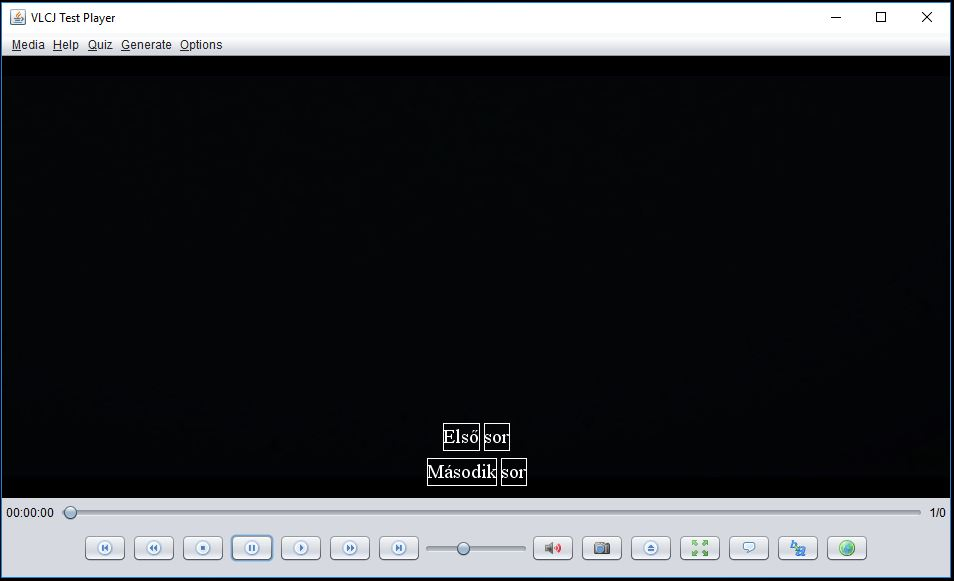
\includegraphics[width=\linewidth]{images/subtitle_boxes.jpg}
  \caption{A befoglaló négyszögek megjelenítve a szavak körül}
  \label{fig:subtitle_boxes}
\end{figure}

A kattintásra történő szöveg visszaadásának megvalósítása az egyes szavakat befoglaló kattintható, láthatatlan téglalapok segítségével történik. Az antialiasing, betűtípus, valamint a betűszín beállítása után a meghívott \textit{calculateSubtitleBoundingBox} végzi el a mondatelemek köré szánt négyszögek kiszámítását. A szavak, valamint az őket körül vevő téglalapok egy kulcs-érték párokat tároló Map-be kerülnek. A map elemeit alkalmazás a kattintás pozíciójának vizsgálatakor elemzi, és amennyiben a kattintás valamely map-ben fellelhető négyszög területén belülre esik, a szoftver visszaadja a hozzá tartozó kulcsot, jelen esetben a \textit{String} objektumot, amely a kattintott mondatelemet tartalmazza. Így tehát lehetőség nyílik a felhasználó egérrel történő kattintásait nyomon követni, és ennek megfelelően elvégezni a szükséges fordítást. A \ref{fig:subtitle_boxes}-as ábrán látható módon, a kód minimális módosításával megjeleníthetők a befoglaló téglalapok, így jól látható, hogy a szoftver mely területekre figyel a felhasználó kattintásai során.

A bemutatott két funkció alkalmazásba történő implementálásával lehetőség nyílt arra, hogy a felhasználó interakcióit a szoftver dinamikusan, a film lejátszása közben kezelje, illetve ennek alapján megfelelő fordításokat végezzen beépített fordító API segítségével.

\section{Feliratok fordítása}

Miután már lehetőségünk van arra, hogy a felhasználó szavakra történő kattintásait nyomon kövessük, a következő lépés ezek lefordítása a kívánt nyelvre. Ehhez szükségesünk van egy fordító \textit{API}-ra, azaz egy alkalmazásprogramozási felületre, amely segítségével megvalósíthatóvá válik a szavak anyanyelvre való átültetése. Ehhez a \textit{Microsoft Translate API} interfészre esett a választásom, mivel az összes alternatíva közül ez az egyetlen ingyenes, bizonyos karakterszám eléréséig. Az \textit{API} működésének lényege, hogy a videólejátszó alkalmazás interneten keresztül elküldi a megadott címre a fordítani kívánt szót, majd innen egy \textit{JSON} formátumú válasz érkezik, ami tartalmazza az összes információt, -beleértve a fordításokat is- amelyet a szerver képes volt előállítani az elküldött információk alapján.
A szolgáltatás többféle fordítási módot is támogat:
\begin{itemize}[noitemsep]
\item fordítás, azaz több mondatos szövegek fordítása
\item transzliteráció, azaz nem latin betűkészletet használó nyelvek átbetűzése
\item szófordítás, azaz egyes szavak szótárazása
\end{itemize}
Az alkalmazás szempontjából az utóbbi lesz megfelelő, mivel ez a funkció lehetővé teszi egy szóhoz tartozó több fordítás megjelenítését is, amely a felhasználó szókincsének bővítésére rendkívül hasznos.

\subsection{Szerverrel történő kommunikáció}
A szolgáltatás használatához regisztrálást követően igényelnem kellett egy egyedi kulcsot, amely a fiókom azonosítását szolgálja. A \textit{TranslateService.java} osztály valósítja meg az információáramlást szerver és kliens között. Mivel az \textit{API} egy másik URL-en képes nyelvfelismerésre is, ezért az osztályba két publikus metódus került. Egy, amely a kiválasztott nyelv esetén hívódik, egy másik pedig amikor a nyelvfelismerés aktív (\ref{lst:adott_nyelv}). 

%caption=Függvény, amely kiválasztott nyelv esetén hívódik, 
\begin{spacing}{1.25}
\begin{lstlisting}[
language=java, 
label={lst:adott_nyelv},
caption={Függvény, amely kiválasztott nyelv esetén hívódik}]

public TranslateResponse[] PostWithGivenLanguages(
    String from,
    String to,
    String string) throws IOException {
        givenLanguageUrl += from + "&to=";
        givenLanguageUrl += to;

        Gson gson = new GsonBuilder()
            .setPrettyPrinting()
            .create();
        return gson.fromJson(createResoponse(string,
            givenLanguageUrl).
        body().string(), TranslateResponse[].class);
    }
\end{lstlisting}
\end{spacing}

Ebben az esetben a metódus három paraméterrel rendelkezik:
\begin{itemize}[noitemsep]
\item String from, a forrásnyelv
\item String to, a célnyelv
\item String string, a fordítandó szöveg
\end{itemize}
Működése közben előállít egy URL-t, amely tartalmazza a fent említett forrás- és célnyelvet, valamint a felhasználáshoz szükséges kulcsot, beégetett módon. A \textit{createResponse} metódus felelős a szerverrel történő kommunikációért, beleértve a kérés elküldését, illetve a válasz átadását is. A kapott \textit{JSON} formátumú szöveget \textit{Gson} segítségével deszerializálja, így jön létre egy \textit{TranslateResponse} tömb, amely a szervertől kapott választ hivatott reprezentálni. Ez tartalmazza az elérhető fordításokból alkotott listát, mellyel tovább dolgozhatunk.

\begin{spacing}{1.25}
\begin{lstlisting}[language=java, label={lst:felismert_nyelv}, caption={Függvény, amely detektált nyelv esetén hívódik}, showstringspaces=false]
public DetectedLanguageResponse[] PostWithLanguageDetection(
    String string) throws IOException {
        Gson gson = new GsonBuilder()
            .setPrettyPrinting()
            .create();
        return gson.fromJson(createResoponse
            (string,
            "https://api.cognitive.microsofttranslator.com
             /detect?api-version=3.0")
                .body().string(),
            DetectedLanguageResponse[].class);
    }
\end{lstlisting}
\end{spacing}

A \ref{lst:felismert_nyelv} ábrán látható a detektált nyelv esetén meghívott függvény. Az előző metódushoz képest annyi különbség fedezhető fel, hogy a paraméterlistában csak a lefordítandó szöveg szerepel, és a POST kérés másik címre fut be. Ezen kívül a feldolgozott \textit{JSON} egy \textit{DetectedTranslateResponse}-okat tartalmazó tömbbe kerül. 

\subsection{Fordítások megjelenítése}
\begin{figure}
  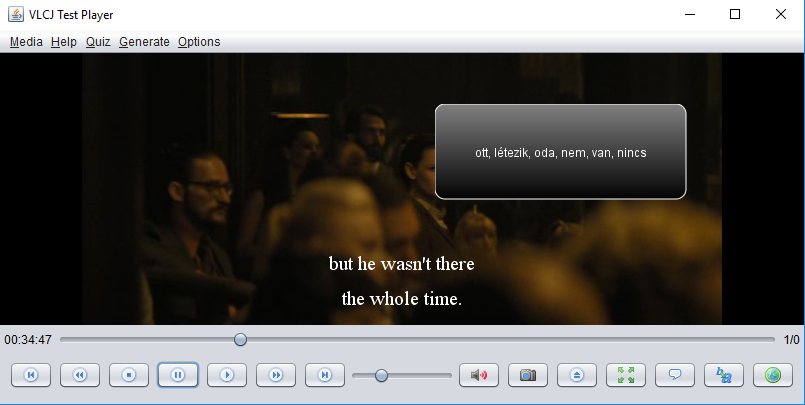
\includegraphics[width=\linewidth]{images/popup.png}
  \caption{A megjelenő felugró ablak}
  \label{fig:popup}
\end{figure}

A fordítások és annak egyéb adatai deszerializáció után kinyerhetők egy-egy objektumtömbből. A következő feladat ezek felhasználóbarát megjelenítése volt. További kritérium, hogy komponens nem szakíthatja meg a videó folytonosságát, illetve nem zavarhatja a nézőt a jelenléte. Mindezek miatt egy felugró ablakot készítettem, amely mondatelemre történő kattintás esetén megjelenik, majd néhány másodperc elteltével eltűnik a képernyőről. Az ablak tartalmazza az aktuális szó összes elérhető fordítását, ha pedig ilyen nem található a \textit{No translations available} felirat jelenik meg. Ennek a megjelenítéséért a \textit{PopupMessageBuilder.java} osztály felelős. Maga az ablak egy \textit{JPanel}-ből származik, melyet a \textit{paintComponent} metódus segítségével rajzol az alkalmazás a képernyőre. A builder osztályt olyan módon készítettem el, hogy segítségével könnyedén, és kényelmesen lehessen felugró ablakokat megjeleníteni a felhasználói a felületen. A \ref{lst:popup}-os ábrán látható módon, pozíció, időtartam, üzenet megadásával jeleníthető meg a komponens. Jelen esetben a kattintás helye felett, három másodperces időtartammal jelenik meg az üzenet, amely a fordítást tartalmazza.

\begin{lstlisting}[caption=A \textit{PopupMessageBuilder} használata, label={lst:popup}, language=java]
new PopupMessageBuilder()
    .at(new Point((int) e.getPoint().getX(), e.getY()
    -(int)(Toolkit.getDefaultToolkit().getScreenSize().height*0.1)))
    .withDelay(3000)
    .withMessage(word.getMeaning())
    .show();

new PopupMessageBuilder()
    .at(new Point((int) e.getPoint().getX(), e.getY()
    -(int) (Toolkit.getDefaultToolkit().getScreenSize().height*0.1)))
    .withDelay(3000)
    .withMessage("No translations available")
    .show();
\end{lstlisting}

A felugró ablak megjelenését filmnézés közben a \ref{fig:popup}-os számú ábrán láthatjuk.
\section{Nyelvek kiválasztása}

\begin{figure}
  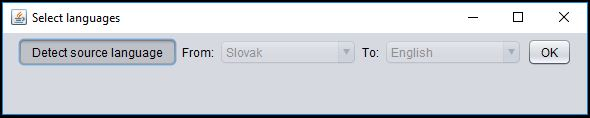
\includegraphics[width=\linewidth]{images/language_selection.jpg}
  \caption{A nyelvválasztó kezelőfelülete}
  \label{fig:language_selection}
\end{figure}

Miután az alkalmazás képes kezelni a fordításokat, a következő lépés a fordítás nyelvének megadása volt. Mivel a szoftver képes nyelvfelismerésre is, ezért a nyelvválasztó funkciót úgy valósítottam meg, hogy a felhasználó képes legyen e funkció be- és kikapcsolására, illetve egyéni nyelvpárok kiválasztására is.  Ez csak azután tehető meg, hogy sikeresen hozzáadunk egy feliratfájlt a lejátszóhoz. Ha ezt megtettük a kezelőfelület elérhető a \textit{Select translator languages} gombra történő kattintással.  Ekkor egy panel nyílik a felhasználó képernyőjére, (\ref{fig:language_selection}) amely egy \textit{JToggleButton}-on kívül kettő \textit{JComboBox}-ot tartalmaz egy \textit{JButton} mellett. Alapesetben a nyelvfelismerés mindig aktív, így a két legördülő listából nem lehet választani. Ez kikapcsolható a \textit{Detect languages} gombra való kattintással. Ekkor elérhetővé válik a két lista is, ahol tetszőlegesen választhatunk a fordító által támogatott nyelvek közül. Választás után az \textit{OK} kattintva az alkalmazás elmenti a kiválasztott elemeket, tehát, ha bezárjuk az ablakot, majd ismét megnyitjuk azt, az eredmény a bezárás előtti állapottal megegyező. Így a megjelenített opciók mindig az aktuális, mentett konfigurációt tükrözik. A fordítás nyelvének megváltoztatása akár filmnézés közben is elvégezhető, nem szükséges hozzá a tartalom újratöltése, azonban minden új feliratfájl lejátszóhoz történő hozzáadása alaphelyzetbe állítja a kiválasztott nyelveket. Az \textit{API} által támogatott nyelvek listája rendkívül széles, a legtöbb ismert nyelvet támogatja.

Mivel az \textit{API} nyelvkódokat használ a nyelvek azonosítására, például \textit{"hu"}, viszont a felhasználó számára megjelenített nyelvek teljes értékű szavak, például \textit{"Hungarian"}, szükség volt ezek összekapcsolására. A nyelv-nyelvkód párokat egy \textit{HashMap}-ben tároljuk kulcs-érték páronként, amelyeket minden egyes nyelvállításkor megvizsgálunk, és  a kulcs alapján az alkalmazás beállítja az annak megfelelő kódot. (\ref{lst:kulcs_ertek}).

\begin{lstlisting}[caption=Aktuális nyelvek beállítása, language=java, label={lst:kulcs_érték}]
while (it.hasNext()) {
    Map.Entry pair = (Map.Entry) it.next();
    if (pair.getKey().equals(fromComboBox.getSelectedItem())) {
        currentFromLanguage = (String) pair.getValue();
    }
    if (pair.getKey().equals(toComboBox.getSelectedItem())) {
        currentToLanguage = (String) pair.getValue();
    }
    it.remove();
}
\end{lstlisting}

Mint említettem, alapesetben a nyelvdetektálás mindig aktív. Ez azt jelenti, hogy a felhasználónak nem kell a nyelvválasztással foglalkoznia, elvégzi ezt helyette az alkalmazás. Emellett ilyen esetben a célnyelv, azaz az a nyelv amire a fordítás történik, mindig a felhasználó számítógépének rendszernyelve, amelyet az alkalmazás a \textit{user.language} változóból olvas ki. Így a a felhasználó számára legkényelmesebben, legkevesebb konfigurációval, mindemellett nagy pontossággal valószínűsíthető, hogy a fordítás mely két nyelv között fog végbemenni, hiszen az \textit{API} nyelvfelismerő funkciója rendkívül megbízható, illetve legtöbbször az operációs rendszer nyelve megegyezik a felszanálója anyanyelvével.

\section{Online feliratok letöltése}

Az alkalmazást a kényelmesebb és felhasználóbarátabb használatért kiegészítettem egy, az alapspecifikáción kívül eső funkcióval, mely az online feliratok keresése és letöltése. Habár korlátlan mennyiségű felirat áll rendelkezésre online, a felhasználók egy része mégsem ismeri ezek beszerzésének módjait. Legfőképpen nekik nyújthat nagy segítséget az implementált funkció, azonban mindenki számára egy kényelmes megoldást kínál. A megvalósításhoz az egyik legnagyobb felirat-adatbázissal rendelkező weboldal saját \textit{API}-ját, az \textit{opensub4j} nevű interfészt hívtam segítségül. A weboldalon történő ingyenes regisztráció után mar használhattam is a felületet.

Első lépésként felvettem egy új függőséget az alkalmazás \textit{pom} fájljába. Ettől kezdve elérhetővé váltak számomra a csomagban definiált osztályok. A funkció implementálását a \textit{SRTSearchFrame.java} osztály tartalmazza. Működése két részből áll: a feliratok keresése, illetve ezek letöltése, kitömörítése.

\subsection{Feliratok keresése}

\begin{figure}[h!]
  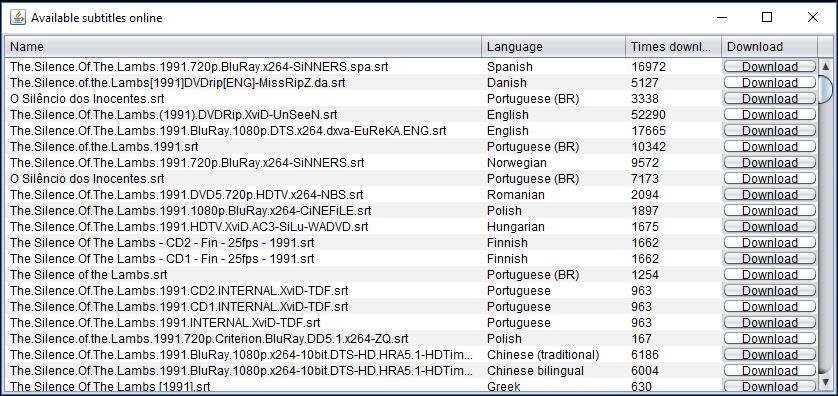
\includegraphics[width=\linewidth]{images/online_search.jpg}
  \caption{Keresési találatokat tartalmazó táblázat}
  \label{fig:online_search}
\end{figure}

A keresőpanel megjeleníthető az alkalmazás alsó kezelőfelületén a \textit{Search for subtitles online} gombra történő kattintással. Ekkor egy egyszerű felület tárul a felhasználó elé. Itt választhat, hogy filmhez, vagy sorozathoz készült feliratot keres. A kettőt azért volt szükséges szétválasztani, mert a két kérés címe mindkét esetben más. A keresési módok között a bal oldalon lévő \textit{JToggleButton}-ra történő kattintással van lehetőség váltásra. Filmek esetében csak a címet, sorozatok esetében pedig a címet, illetve lehetőség szerint az évadot, epizódot kell megadnunk. A \textit{Search} gombra történő kattintással elindíthatjuk a keresést, melyet egy függvény végez, ami a \ref{lst:search}-es kódrészleten látható. A keresés nyelvét egy rendszerváltozóból kapja, a név-évad-epizód hármast pedig a megfelelő \textit{JTextField}-ekből. Ezután a \textit{.srt} kiterjesztésre való szűrés megy végbe. 

\begin{spacing}{1.25}
\begin{lstlisting}[caption=Feliratok keresése sorozatokhoz valamint filmekhez, label={lst:search}, language=java]
//if it is a serial
if (isSerial.isSelected()) {
    subtitles = osClient.searchSubtitles(
    System.getProperty("user.language"),
    nameTextField.getText(),
    seasonTextField.getText(),
    episodeTextField.getText())
        .stream()
        .filter(sub -> sub.getFormat()
        .equals("srt"))
        .collect(Collectors.toList());
//if it is a movie
} else {
    //...
}
\end{lstlisting}
\end{spacing}

A művelethez természetesen internetkapcsolat szükséges, ennek hiányában az alkalmazás hibaüzenetet jelenít meg a felhasználónak, az \textit{An unexpected error has occurred. Please check your internet connection.} szöveggel. Mivel az \textit{API} képes kezelni a hiányos, esetleg hibás keresési feltéteket, így legtöbbször elég a film vagy sorozat címének egy részét is megadni. Amennyiben a keresés sikeres egy táblázat tárul elénk, amely az összes megtalált felirat közül -az alkalmazás kompatibilitása miatt-, csak a \textit{.srt} kiterjesztésűeket tartalmazza. Ez megtekinthető a \ref{fig:online_search}-os ábrán. A táblázatban megjelenik a feliratfájl neve, nyelve, letöltéseinek száma, valamint egy \textit{Download} gomb, mely a felirat letöltését indítja el.

\subsection{Feliratok letöltése}

\begin{spacing}{1.25}
\begin{figure}
  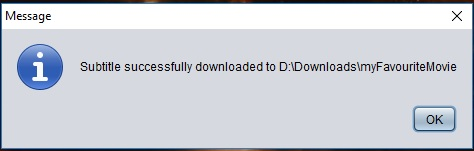
\includegraphics[width=\linewidth]{images/downloaded_sub.jpg}
  \caption{A letöltés helyét megjelenítő információs panel}
  \label{fig:downloaded_sub}
\end{figure}
\end{spacing}

Miután megtaláltuk a számunkra megfelelő feliratot, kattintsunk a letöltés gombra. Sikeres letöltés esetén egy \textit{JOptionPane} jelenik meg a képernyőn, amely tájékoztatja a felhasználót a letöltött fájlt tartalmazó könyvtárról (\ref{fig:downloaded_sub}). Ez alapértelmezetten a \textit{user.dir} rendszerváltozóból kerül kiolvasásra, azonban amennyiben bármilyen médiafájl már importálásra került a lejátszóba, a letöltés annak a fájlnak a tartalmazó könyvtárába kerül.
A letöltést a \textit{Wget.java} osztály végzi, amely egyetlen metódust tartalmaz. Ez paraméterként a mentendő fájl URL-jét, valamint egy útvonalat vár, ahova a kiírás történik. Törzsében egy \textit{HttpURLConnection}-ön keresztül egy \textit{GET} kérést indít, amely \textit{InputStream}-ként adja át az adatokat. Mivel az állomány tömörített, ezért \textit{ArchiveInputStream} használatára is szükség van, amely a \textit{stream}-et megfelelően kezeli. A metódus létrehoz egy \textit{OutputStream}-et, amelybe átkonvertálja az \textit{InputStream} tartalmát. Végül mindkét \textit{stream}-et lezárja. E folyamat segítségével az alkalmazás képes a letöltött állományt kitömörítve elmenteni a felhasználó merevlemezére, amely így már azonnal importálható a lejátszóba.
\section{Adatbázis műveletek}


\begin{spacing}{1.25}
\begin{figure}[h!]
  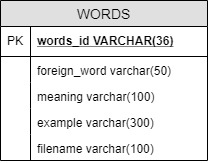
\includegraphics[width=.5\linewidth]{images/entity.jpg}
  \centering
  \caption{Adatbázis struktúra}
  \label{fig:entity}
\end{figure}
\end{spacing}\todo[inline]{ehelyett az elmosódott táblázat helyett én inkább csinálnék egy latex-es table-t, de rád bízom. Ha átszerkeszted akkor táblázatként is hivatkozz rá!}

Ahhoz, hogy az alkalmazás további funkcióit, beleértve a pdf fájl, illetve tudásellenőrző teszt generálását implementálni tudjuk szükségünk van egy adatbázisra, amely az eddig elvégzett fordításokat tartalmazza kiegészítő adatokkal. Ehhez egy igazán könnyűsúlyú, egyszerűen telepíthető és használható adatbázist, a \textit{H2} adatbázist vettem segítségül. Használatához csupán a megfelelő függőséget kellett az alkalmazás \textit{.pom} állományába importálnom. Az adatbázist \textit{liquibase} segítségével hoztam létre. Az ehhez szükséges \textit{changelog.xml} mellett létrehoztam egy \textit{create-table.xml} fájlt, amely alapján a \textit{liquibase} megalkotja az adatbázistáblát, amely a \ref{fig:entity} számú ábrán látható. Ez a leírófájl 
úgynevezett \textit{changeSet}-eket tartalmaz, melyek adatbázis műveleteket írnak le, és a \textit{liquibase} sorban, egymás után hajt végre ezeket az adatbázison. Az első létrehozza a táblát, ha még az nem volt előtte létrehozva, a második pedig hozzáadja az elsődleges kulcsot, amely jelen esetben a \textit{words\_id}. Ez egy egyedi azonosító, melynek ismeretében pontosan meghatározható bármely rekord az adatbázisban. Formátuma \textit{UUID}, ami egy 36 karakter hosszú egyedi karakterlánc. A tábla további elemei:
\begin{itemize}
\item \textbf{ foreign\_word}, a mondatelem, amelyre a felhasználó kattintott, legfeljebb 50 karakter hosszú
\item \textbf{meaning}, a mondatelem jelentése(i), legfeljebb 100 karakter hosszú
\item \textbf{example}, példamondat, amely a mondatelem kontextusából kerül ki, legfeljebb 300 karakter hosszú
\item \textbf{filename}, feliratfájl neve, amelyben az aktuális mondatelem szerepelt, legfeljebb 100 karakter hosszú
\end{itemize}

Miután a tábla elkészült, lehetőség nyílik azon a szükséges adatbázis műveletek végrehajtására. Az objektumok a nyelvfordítás elvégeztével kerülnek be az adatbázisba. Amennyiben már megtalálhatóak ott, nem történik újbóli mentés. Mivel az alkalmazás működtetéséhez csupán néhány lekérdezésre, és beszúrásra volt szükségem, egyszerű \textit{jdbc} műveletek használata mellett döntöttem. Ezek a \textit{WordService} osztályban kerültek implementálásra. Megvalósított műveletek:
\begin{itemize}
\item \textbf{create}, a szavak adatbázisba történő mentésére szolgál
\item \textbf{getAllByFilename}, visszatér az összes szóval, melyek fájlnevei megegyeznek a paraméterben kapott fájlnévvel
\item \textbf{isAlreadySaved}, visszatérési értéke igaz vagy hamis, attól függően, hogy a paraméterben kapott szó megtalálható-e már az adatbázisban
\item \textbf{deleteAll}, törli az összes rekordot az adatbázisból
\item \textbf{getAll}, visszetér az összes adatbázisban található rekorddal
\end{itemize}
Egy metódus felépítése a \ref{lst:deleteAll}-es kódrészleten látható, és a következőképpen működik: először létrehoz egy \textit{Connection} kapcsolatot, amely az adatbázisfájl, és a hozzá tartozó azonosítók (felhasználónév, jelszó) ismeretében lehetséges. Majd ezen végrehajt egy műveletet, melyet \textit{SQL} nyelven kell megadnunk a \textit{jdbc}-nek. Amennyiben a művelet végrehajtása közben kivétel dobódott, az alkalmazás egy \textit{JOptionPane} hibapanelt jelenít meg a képernyőn, a felhasználó tudtára adva, hogy váratlan hiba keletkezett a folyamat közben.


\begin{spacing}{1.25}
\begin{lstlisting}[caption=Implementált deleteAll metódus, language=java, label={lst:deleteAll}, ]
public void deleteAll() {
    try (Connection connection = DriverManager
    .getConnection("jdbc:h2:file:~/basicvlcj", "sa", "");
        Statement stat = connection.createStatement()) {
            stat.executeUpdate("DELETE FROM WORDS");
    } catch (SQLException e) {
        JOptionPane.showMessageDialog(JOptionPane.getRootFrame(),
        "An unexpected error has occurred",
        "Error",
        JOptionPane.ERROR_MESSAGE);
    }
}
\end{lstlisting}
\end{spacing}

Az imént említett függvények megvalósítása után egyszerűen lekérdezhetővé váltak a többi funkció által igényelt adatok. Így ezen komponensek implementálásával folytattam a fejlesztést.
\section{Szótár generálása ismeretlen szavakból}

\begin{figure}[h!]
  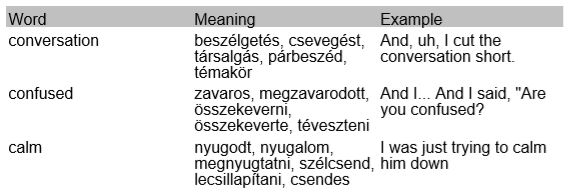
\includegraphics[width=\linewidth]{images/pdf.jpg}
  \caption{Ismeretlen szavakból generált szótár}
  \label{fig:pdf}
\end{figure}

Az alkalmazás képes fordítások megjelenítésére, valamint adatbázisba való elmentésükre, így a következő megvalósított funkció a szótárgenerálás volt. A szoftver az adatbázisból lekérdezés segítségével kinyeri a szükséges adatokat, majd ezekből egy \textit{.pdf} kiterjesztésű szószedetet állít elő. A szótár tartalmazza az ismeretlen szót, azaz a mondatelemet, amire a felhasználó kattintott, a jelentését vagy jelentéseit, valamint a kontextust, a mondatot, amelyben a kattintott elem szerepelt (\ref{fig:pdf}).

Először szükség volt egy függőség importálására az alkalmazás \textit{pom} fájljába. A választás az \textit{itextpdf} \textit{API}-jára esett, mely segítségével az említett funkcionalitás megvalósítása maradéktalanul kivitelezhető. Ezután a \textit{PDFGeneratorService} osztályt alkottam meg, amely a fájlgenerálásért felelős. Ebben található a \textit{createDictionary} metódus, amely az adatbázis adataiból a konkrét szószedetet kreálja. Egy új \textit{Document} objektum létrehozása után a \textit{PdfWriter} a dokumentum és egy \textit{FileOutputStream} segítségével hozza létre a merevlemezen a tényleges fájlt. A fájl neve alapesetben az aktuális feliratfájl nevével egyezik meg. Ezután egy táblázat kerül a dokumentumba, mely 3 oszlopból áll. A táblázat fejlécét az \textit{addTableHeader} függvény készíti el, így az tartalmazza a oszlopok feliratait, valamint egy világosszürke hátteret állít be neki. Az adatbázisból elkérjük az aktuális fájlnév alapján a rekordokat, majd ezen végig iterálunk, olyan módon, hogy minden rekordból egy \textit{Word} objektumot készítünk, amit pedig új sorként adunk a táblázathoz. A bejárás végeztével hozzáadjuk a táblázatot a dokumentumhoz, majd bezárjuk azt, ezzel lezárva a fájlt, és elérhetővé téve azt a felhasználónak. A folyamat forráskódját a \ref{lst:pdf} ábra tartalmazza.

\begin{spacing}{1.25}
\begin{lstlisting}[caption=PDF fájl megalkotása, language=java, label={lst:pdf}]
document.open();
PdfPTable table = new PdfPTable(3);
addTableHeader(table);

for (Word word : new WordService()
.getAllByFilename(
PlayerControlsPanel.actualSubtitleFile.getName())) {
    addRow(table,
    word.getForeignWord(),
    word.getMeaning(),
    word.getExample());
}
document.add(table);
document.close();
\end{lstlisting}
\end{spacing}

E funkció megvalósításával lehetőség nyílt a felhasználó számára, hogy a neki ismeretlen szavakat és ezek jelentését kényelmesen hordozható formában elmentse. Ezáltal egy későbbi alkalommal, esetleg tanulás közben e szavak memorizálására fokozott figyelmet fordíthat, anélkül, hogy a kigyűjtésükhöz bármiféle plusz eszköz szükségeltetett volna, hiszen mindez filmnézés, szórakozás közben történt.
\section{Tudásellenőrző kvíz generálása ismeretlen szavakból}

A funkció célja, hogy egy film végignézése után a felhasználó játékos módon ellenőrizni tudja, hogy az általa ismeretlen szavak mennyire rögzültek filmnézés alatt.
Erre egy kvíz tökéletes megoldás, hiszen így gyorsan, könnyedén, alternatívák közül választva érhet el a felhasználó egy adott pontszámot, amely a filmnézés közben szerzett nyelvtudását tükrözi. Egy ilyen tudásellenőrző még jobban ösztönözheti kitöltőjét az ismeretlen szavak elsajátítására, hiszen a kvízben elért magas pontszám sikerélménnyel párosulhat.

\begin{figure}[h!]
  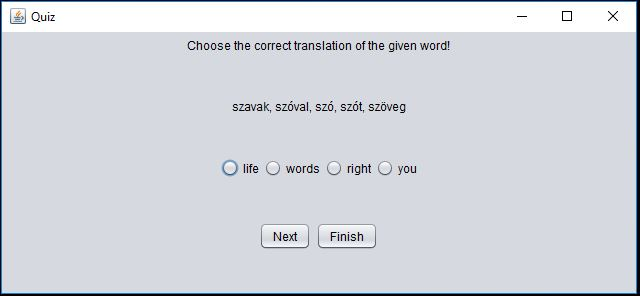
\includegraphics[width=\linewidth]{images/quiz.jpg}
  \caption{Egy a kvízben előforduló kérdés}
  \label{fig:quiz}
\end{figure}

Implementálás során egy \textit{Quiz.java} osztályt készítettem, amely a \textit{JFrame} osztály leszármazottja és képes a kvíz előállítására az adatbázisból kapott adatokból, valamint ennek megjelenítésére, kezelőfelület biztosítására. Ezen belül található egy beágyazott osztály, a \textit{RadioQuestion}, amely egy feleletválasztós kérdést reprezentál, őse a \textit{JPanel} osztály. A működési elv egyszerű: a kvíz ablaka mindig egy kérdést jelenít meg, amit helyes válasz esetén cserél, rossz válasz esetén pedig felugró ablakkal jelzi, hogy a megadott válasz helytelen. Egy kérdés mindig tartalmazza az utasítást, alatta a fordítást vagy fordításokat, lentebb pedig a választási lehetőségeket. A panel alján a \textit{Next}, valamint a \textit{Finish} gombok találhatók meg (\ref{fig:quiz}). A megoldás bejelölése után a \textit{Next}-re kattintva új kérdés következik, a \textit{Finish}-re kattintva pedig befejezhetjük a kvízt, amelyet egy pontösszesítő ablak jelez. A tudásfelmérő elindítható az alkalmazás felső menüsorából, a \textit{Quiz/Take quiz...} menüpontot választva. Ahhoz, hogy a szoftver helyesen tudja megalkotni a kérdéseket alternatívákkal, legalább 6 megfelelő rekordot kell tartalmaznia az adatbázisnak. Amennyiben ez nem teljesül a felhasználót erről egy ablak tájékoztatja, egyébként megjelenik a kvíz ablaka, benne az első kérdéssel.

\begin{spacing}{1.25}
\begin{lstlisting}[caption=Kérdések előállítása, language=java, label={lst:questions}]
words = wordService.getAllByFilename(
   PlayerControlsPanel
   .actualSubtitleFile.getName());

questions = new RadioQuestion[words.size()];
    for (int i = 0; i < questions.length; i++) {
        questions[i] = new RadioQuestion(
            generateRandomAnswers(i),
            words.get(i).getMeaning(),
            words.get(i).getForeignWord(),
            this);
}
\end{lstlisting}
\end{spacing}

  \begin{figure}[h!]
\centering
  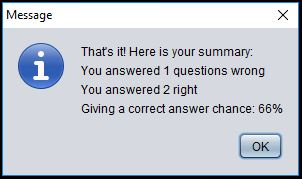
\includegraphics[width=.5\linewidth]{images/summary.jpg}
  \caption{Pontösszesítő ablak}
  \label{fig:summary}
\end{figure}

 A kérdések a \textit{Quiz.java} osztály konstruktorában kerülnek előállításra, és egy tömbben tárolódnak. Először az adatbázisban tárolt szavakat fájlnév szerint lekérdezi, amiket egy listába ment el. Majd ugyanilyen mérettel létrejön egy tömb a kérdés objektumoknak. A függvény végig iterál a tömbön, és minden helyre egy kérdés objektumot hoz létre az alábbi paraméterekkel: Az első paraméter a \textit{generateRandomAnswers} függvény, ami egy \textit{String} tömbbel tér vissza, mely három véletlenszerű alternatívát és egy megoldást tartalmaz. A következő paraméterek az eredeti szó jelentése(i), az eredeti, idegen szó, valamint maga az \textit{Quiz} objektum (\ref{lst:questions}-es kódrészlet). Az alkalmazás ettől kezdve váltogatja a kérdéseket, amikor pedig mindre válaszoltunk egy összesítő ablakot jelenít meg, amelyben láthatjuk hányszor válaszolunk helyesen, és hányszor helytelenül (\ref{fig:summary}-es ábra).
 

A bemutatottak alapján megállapítható, hogy a kvíz generálás funkció segíthet rögzíteni, vagy akár elmélyíteni a filmezés közben szerzett információkat, mindezt szórakozással egybekötve.

\chapter*{Nyilatkozat}
%Egy üres sort adunk a tartalomjegyzékhez:
\addtocontents{toc}{\ }
\addcontentsline{toc}{section}{Nyilatkozat}
%\hspace{\parindent}

% A nyilatkozat szövege más titkos és nem titkos dolgozatok esetében.
% Csak az egyik tipusú myilatokzatnak kell a dolgozatban szerepelni
% A ponok helyére az adatok értelemszerûen behelyettesídendõk es
% a szakdolgozat /diplomamunka szo megfeleloen kivalasztando.


%A nyilatkozat szövege TITKOSNAK NEM MINÕSÍTETT dolgozatban a következõ:
%A pontokkal jelölt szövegrészek értelemszerûen a szövegszerkesztõben és
%nem kézzel helyettesítendõk:

\noindent
Alulírott \makebox[4cm]{\dotfill} szakos hallgató, kijelentem, hogy a dolgozatomat a Szegedi Tudományegyetem, Informatikai Intézet \makebox[4cm]{\dotfill} Tanszékén készítettem, \makebox[4cm]{\dotfill} diploma megszerzése érdekében.

Kijelentem, hogy a dolgozatot más szakon korábban nem védtem meg, saját munkám eredménye, és csak a hivatkozott forrásokat (szakirodalom, eszközök, stb.) használtam fel.

Tudomásul veszem, hogy szakdolgozatomat / diplomamunkámat a Szegedi Tudományegyetem Informatikai Intézet könyvtárában, a helyben olvasható könyvek között helyezik el.

\vspace*{4cm}

\begin{tabular}{lc}
Szeged, \today\
\hspace{2cm} & \makebox[6cm]{\dotfill} \\
& aláírás \\
\end{tabular}


\vspace*{2cm}

%A nyilatkozat szövege TITKOSNAK MINÕSÍTETT dolgozatban a következõ:

%\noindent
%Alulírott \makebox[4cm]{\dotfill} szakos hallgató, kijelentem, hogy a dolgozatomat a Szegedi Tudományegyetem, Informatikai Intézet \makebox[4cm]{\dotfill} Tanszékén készítettem, \makebox[4cm]{\dotfill} diploma megszerzése érdekében.

%Kijelentem, hogy a dolgozatot más szakon korábban nem védtem meg, saját munkám eredménye, és csak a hivatkozott forrásokat (szakirodalom, eszközök, stb.) használtam fel.

%Tudomásul veszem, hogy szakdolgozatomat / diplomamunkámat a TVSZ 4. sz. mellékletében leírtak szerint kezelik.

%\vspace*{1cm}

%\begin{tabular}{lc}
%Szeged, \today\
%\hspace{2cm} & \makebox[6cm]{\dotfill} \\
%& aláírás \\
%\end{tabular}

\chapter*{Köszönetnyilvánítás}
\addcontentsline{toc}{section}{Köszönetnyilvánítás}

Ezúton szeretnék köszönetet mondani \textbf{X. Y-nak} ezért és ezért \ldots




%Irodalomjegyzek
\bibliography{mybib}{}
\bibliographystyle{plain}



\end{document}